\begin{figure*}[h]
\centering

\def\picScale{0.08}    % define variable for scaling all pictures evenly
\def\plotScale{0.2}    % define variable for scaling all plots evenly
\def\colWidth{0.22\linewidth}

\begin{tikzpicture} %[every node/.style={draw=black}]
% \draw[help lines] (0,0) grid (4,2);
\matrix [row sep=0cm, column sep=0cm, style={align=center}] (my matrix) at (0,0) %(2,1)
{
& \node (q1) {(a) $\Delta l = 0, \Delta \phi = 0$}; & \node (q2) {(b) $\Delta l = 5\text{mm}, \Delta \phi = 0$}; & \node (q3) {(c) $\Delta l = 0, \Delta \phi = 20^\circ$}; & \node (q4) {(d) $\Delta l = 5\text{mm}, \Delta \phi = 20^\circ$};

\\

&
\node[style={anchor=center}] {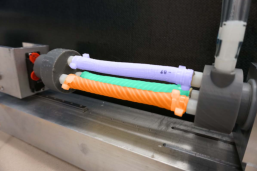
\includegraphics[width=\colWidth]{figures/photos/s0w0pic_colored.pdf}}; %\fill[blue] (0,0) circle (2pt);
&
\node[style={anchor=center}] {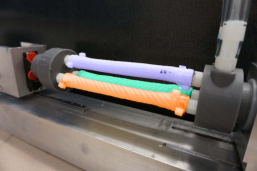
\includegraphics[width=\colWidth]{figures/photos/s5w0pic_colored.pdf}}; %\fill[blue] (0,0) circle (2pt);
&
\node[style={anchor=center}] {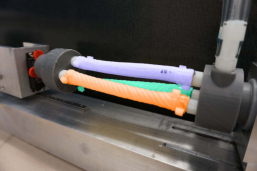
\includegraphics[width=\colWidth]{figures/photos/s0w20pic_colored.pdf}}; %\fill[blue] (0,0) circle (2pt);
&
\node[style={anchor=center}] {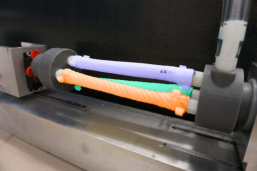
\includegraphics[width=\colWidth]{figures/photos/s5w20pic_colored.pdf}}; %\fill[blue] (0,0) circle (2pt);

\\

\node[rotate=90] (ylabel) {Moment, $M^{\hat{z}_e}$ (N-m)};
&
\node[style={anchor=center}] {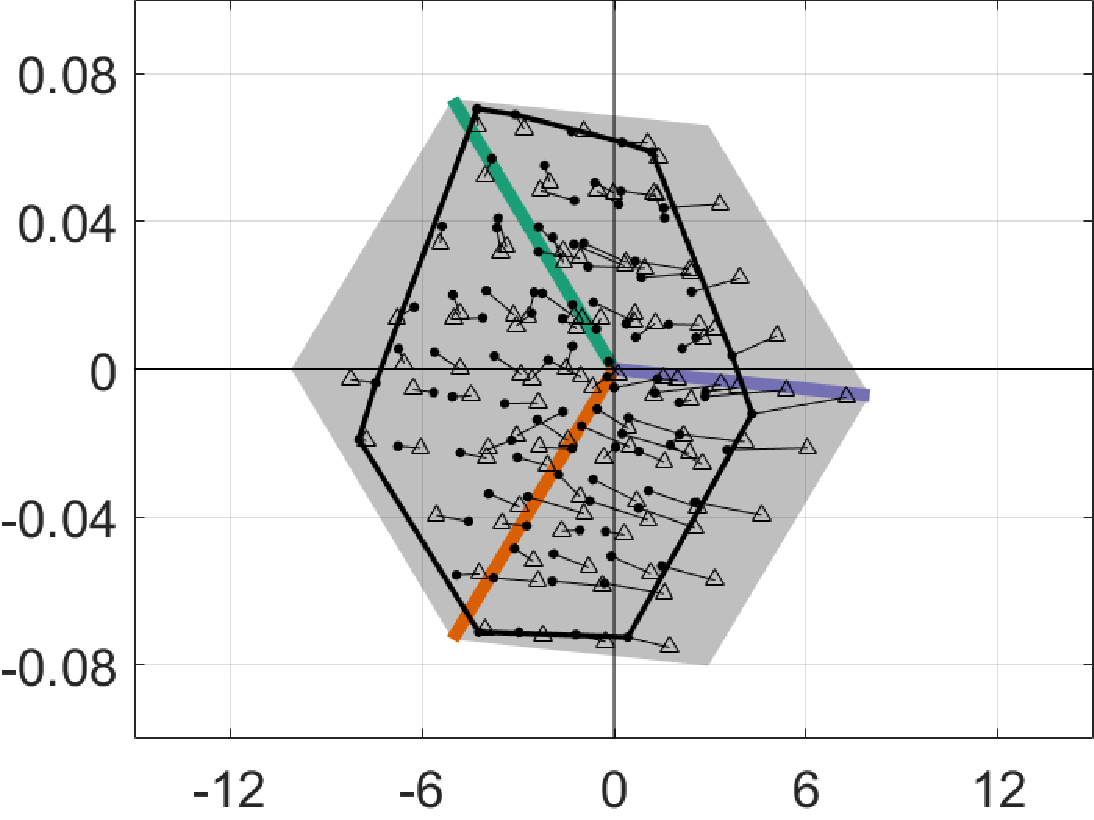
\includegraphics[width=\colWidth]{figures/plots3/s0w0.pdf}}; %\fill[blue] (0,0) circle (2pt);
&
\node[style={anchor=center}] {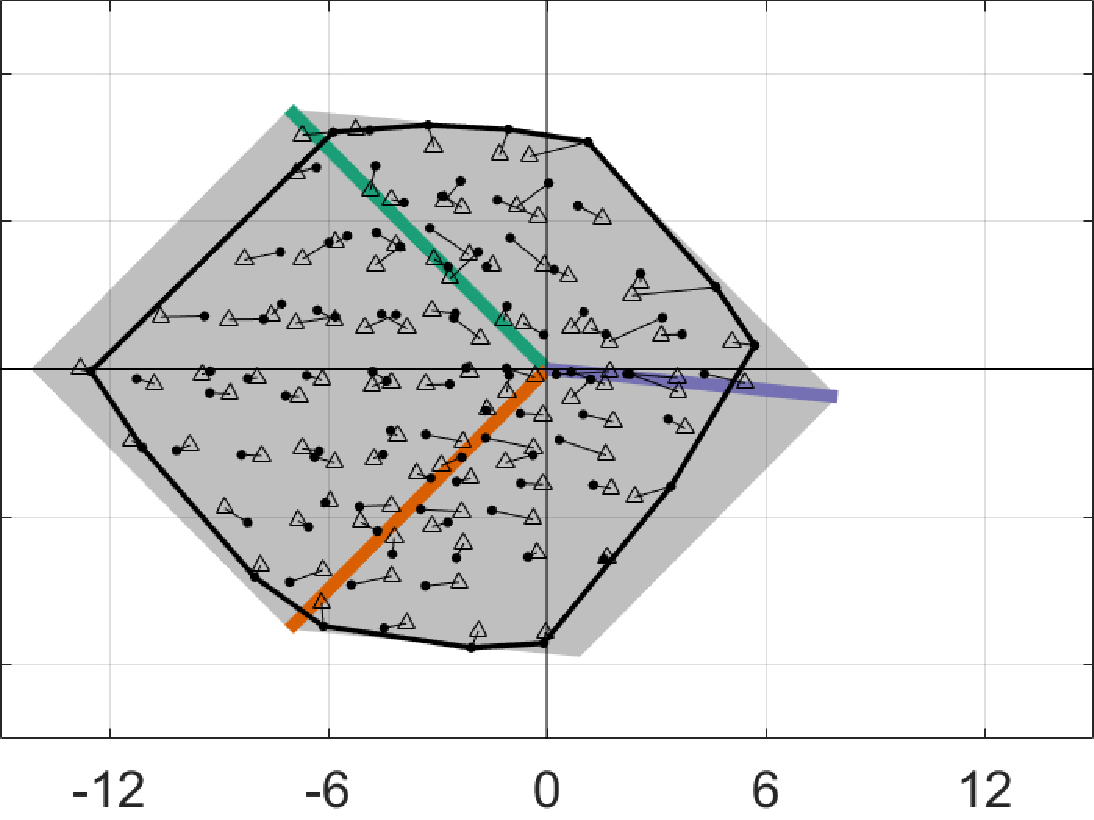
\includegraphics[width=\colWidth]{figures/plots3/s5w0.pdf}}; %\fill[blue] (0,0) circle (2pt);
&
\node[style={anchor=center}] {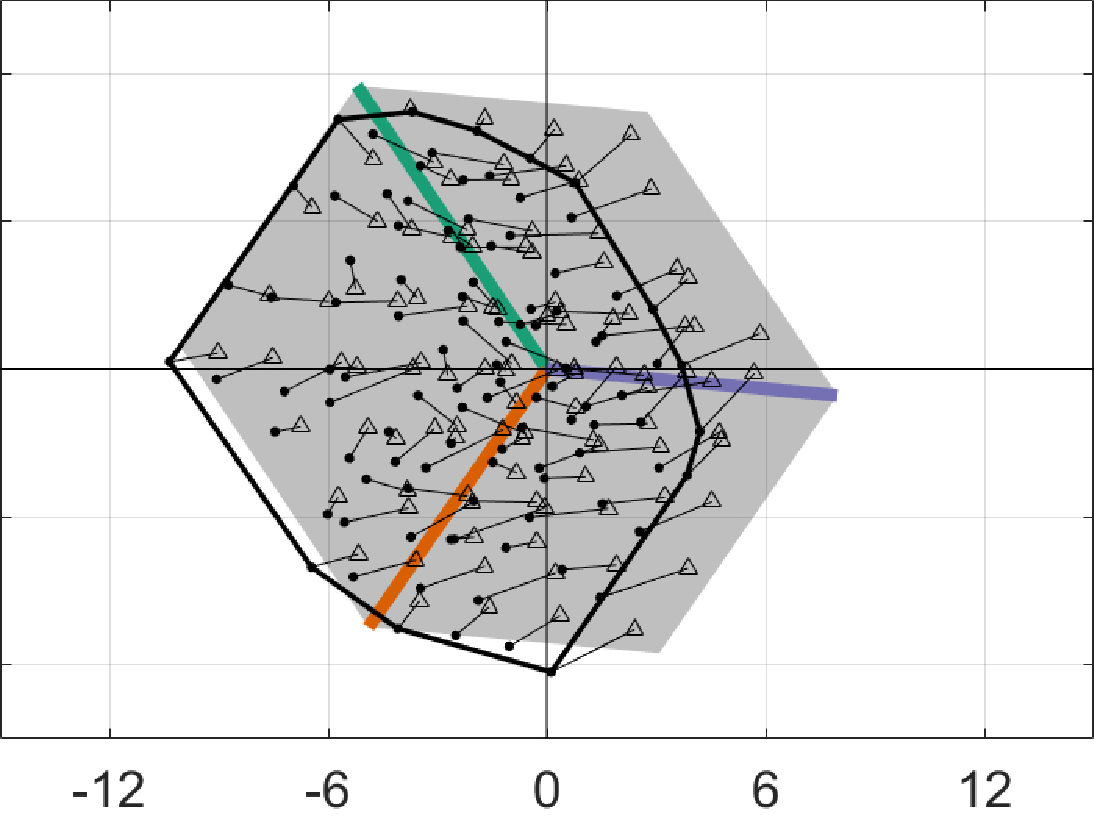
\includegraphics[width=\colWidth]{figures/plots3/s0w20.pdf}}; %\fill[blue] (0,0) circle (2pt);
&
\node[style={anchor=center}] {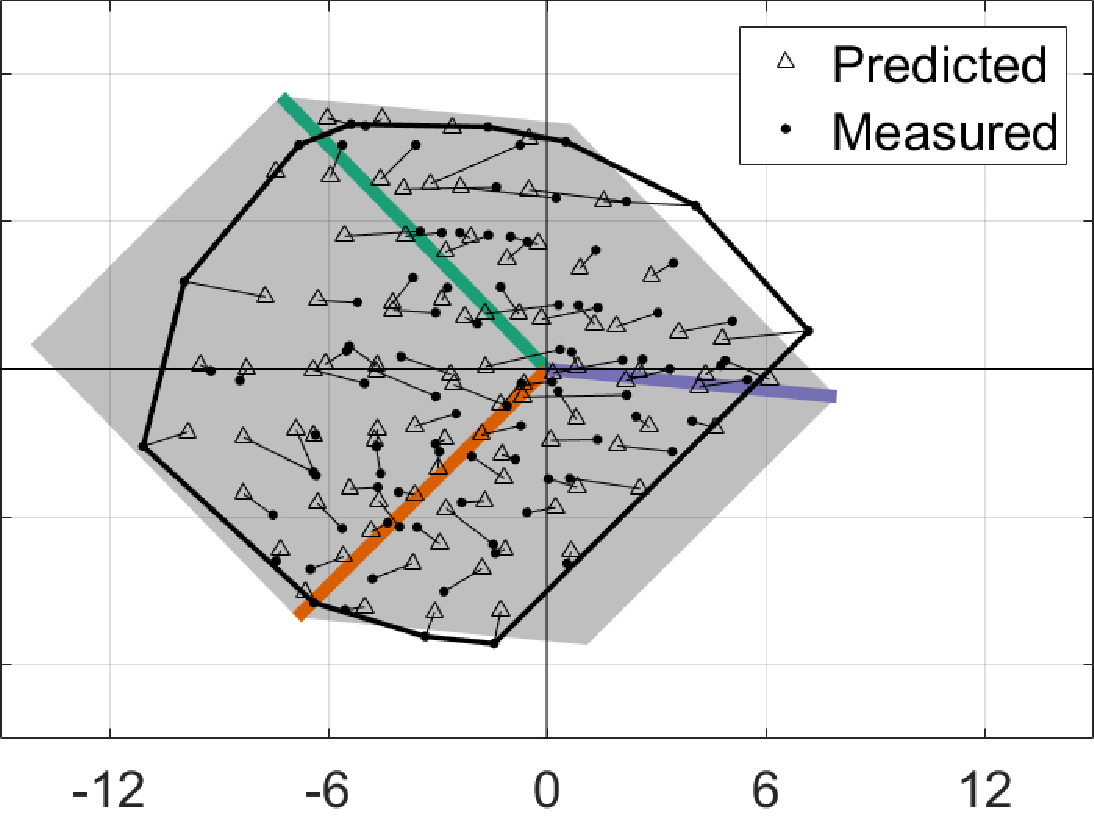
\includegraphics[width=\colWidth]{figures/plots3/s5w20.pdf}}; %\fill[blue] (0,0) circle (2pt);

\\

& \node (xlabel1) {Force, $F^{\hat{z}_e}$ (N)}; & \node (xlabel2) {Force, $F^{\hat{z}_e}$ (N)}; & \node (xlabel3) {Force, $F^{\hat{z}_e}$ (N)}; & \node (xlabel4) {Force, $F^{\hat{z}_e}$ (N)};

\\
};
\end{tikzpicture}

\caption{For four different deformed configurations (top row), we compare the predicted and the measured forces for the parallel combination of three FREEs (bottom row). 
\revcomment{2.6}{Data points and predictions corresponding to the same input pressures are connected by a thin line, and the convex hull of the measured data points is outlined in black.}
The Trial 1 data is overlaid on top of the theoretical force zonotopes (grey areas) for each of the four configurations.
Identical colors indicate correspondence between a FREE and its resulting force/torque direction.}
\label{fig:results}
\end{figure*}






% & \node (a) {(a)}; & \node (b) {(b)}; & \node (c) {(c)}; & \node (d) {(d)};

